\documentclass{bioinfo}
\copyrightyear{2011}
\pubyear{2011}
\raggedend
\usepackage{hyperref}
\hypersetup
{ % We don't want the hideous colored borders around the hyperlinks
  colorlinks=false,
  pdfborder={0,0,0},
}

\begin{document}
\firstpage{1}

\title[ParsEvalMPI]{ParsEvalMPI: comparison of gene structure annotations in parallel}
\author[Daniel S. Standage]{Daniel S. Standage}
\address{Department of Genetics, Development, and Cell Biology}

\history{Submitted on May 3, 2011}

\maketitle

\begin{abstract}
\noindent Accurate gene structure annotation is a fundamental but somewhat elusive goal of genome projects. Genomes typically undergo several cycles of re-annotation. In many cases, it is not only different versions of annotations that need to be compared but also different sources of annotation of the same genome, derived from distinct gene structure prediction workflows. Such comparisons are of interest to annotation providers, prediction software developers, and end-users alike, who all need to assess what is common and what is different between distinct annotation sources.

Building on previous work, I implemented ParsEvalMPI, a C program for comparing gene structure annotations in parallel. Source code for ParsEvalMPI can be accessed online at \url{http://gremlin4.gdcb.iastate.edu:8080/source/xref/pempi/}.
\end{abstract}

\section*{Introduction}
Genome projects typically involve a prolonged annotation effort that continues well beyond the initial release of the genome sequence. The majority of this effort is spent identifying the genome-encoded genes, and consequently the development and evaluation of software tools for predicting gene structures on the genome scale remains an active and critical area of research. Such tools are typically tested on genomic regions with extensive high-quality manual curation, allowing the comparison of the computed predictions with a reliable reference. Even when high-quality reference annotations are not available, tool developers may need to compare gene structures predicted by their tool with those predicted by another tool to identify similarities and differences. Automation of these types of comparisons is crucial to the software development and evaluation process. 

An additional concern stems from the fact that in the context of whole-genome annotation, gene structure annotations are not static. As genome sequencing projects gather novel sequence data, in particular through more in-depth transcriptome sequencing, and as curation efforts expand, successive versions of whole genome annotations will accumulate. Automated comparison of these different annotation versions is necessary to quantify and summarize the differences.

With direction from my advisor, I previously implemented a software application for comparing two sets of gene structure annotations. This software, called ParsEval, was implemented in Perl and had external dependencies, one of which limited its use to specific Linux distributions. To improve the performance and portability of this program, I decided to implement a parallel version of ParsEval.

Here I present ParsEvalMPI, a re-implementation of ParsEval in C that has been parallelized using MPI libraries. I provide a basic overview of the program and its implementation, as well as an evaluation with regards to performance, data distribution, load balancing, and scalability.

\section*{Notation}
Let $G = G_1 G_2 G_3 ... G_N$ represent a sequence of genomic DNA of length $N$ (measured in \textit{nucleotides} or \textit{base pairs}). A gene is a subsequence $g = G_{i} G_{i+1} ... G_{j-1} G_{j}$ of $G$ that encodes instructions for synthesizing a protein. The goal of a gene prediction algorithm is to identify all subsequences of $G$ that correspond to a gene and to describe the function of each nucleotide in that gene. These predictions are called \textit{gene annotations}. A gene annotation may or may not be correct: indeed, different gene prediction algorithms will produce difference annotations for the same genomic sequence.

Let $Refr = \{ r_1, r_2, ..., r_{m_r} \}$ and $Pred = \{ p_1, p_2, ..., p_{m_p} \}$ be two sets of gene structure annotations derived from two different gene prediction algorithms: a reference set and a prediction set, respectively. For an annotation $a_i$ from either set, let $startpos(a_i)$ and $endpos(a_i)$ be the starting and ending positions (respectively) of the corresponding gene prediction, and let $range(a_i)$ be the range of indices between $startpos(a_i)$ and $endpos(a_i)$, inclusive. We now define a \textit{locus} as a maximal subsequence $l = G_{i} G_{i+1} ... G_{j-1} G_{j}$ of G such that each position of $l$ is in the range of at least one gene annotation $a_i \in Refr \cup Pred$. Typically, we expect one annotation from the reference and one annotation from the prediction in each locus, but there are occasional exceptions: a locus with only one annotation, or a locus in which one or more annotations from one set overlap with multiple annotations from the other set.

Finally, let $p$ be the number of processors executing the parallel program, $rank \in 0,1,2,...p-1$ be the identifier of the current process, and $comm$ be the entire collection of $p$ processors executing the program.

\begin{figure*}
  \begin{center}
    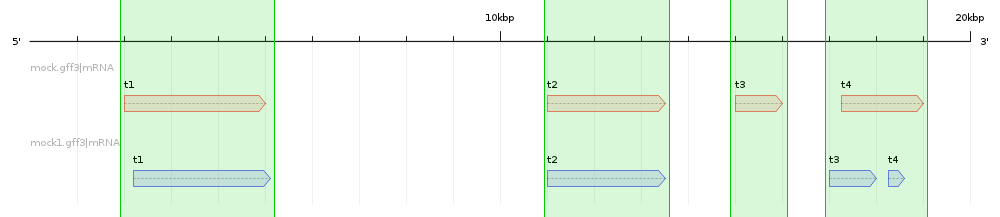
\includegraphics[width=500px]{data.png}
  \end{center}
  \caption{Here the horizontal axis represents a sequence of genomic DNA, and the two rows of boxes represent annotations derived from two different gene structure prediction algorithms. We defined a \textit{locus} as a maximal subsequence where at least on of the annotation sets has predicted a gene. The loci are highlighted in green for this example.}
\end{figure*}

\begin{methods}
\section*{Methods}
ParsEvalMPI is implemented in C and uses, in addition to several standard libraries, an external library called \textit{GenomeTools} (\url{http://genometools.org/libgenometools.html}). This library provides the data parsers and dynamic data structures necessary when parsing gene structure annotation data. Unfortunately, this library did not compile on the older version of Red Hat Linux running on the HPC-class computer, so I used the supercomputing resources of my undergraduate institution to implement this class project. As a result, I also had to install the Jumpshot program manually so as to enable load balancing analysis. It took some time to figure everything out, but in the end I was able to get everything that my program needed installed.

The ParsEvalMPI program can be broken down into three primary phases: the \textit{delegation} phase, in which the program determines the optimal distribution of work (time) and data (space) among the processors; the \textit{local analysis} phase, in which the program calculates comparison statistics for each locus independently; and the \textit{global analysis} phase, in which the program does a brief summary analysis of the entire DNA sequence. A more detailed descriptions of these phases is provided hereafter.

\subsection*{Delegation}
The purpose of the delegation phase is to determine the optimal distribution of of data between the $p$ processors executing the program. Obtaining a theoretically optimal distribution is improbable (if not impossible) and quite unnecessary in practice, but there are several possible approaches to approximate an optimal distribution of data and work.

\begin{enumerate}
  \item The first and simplest approach is to assume no memory constraints an to distribute all data on all processors. This approach is certainly feasible for data sets of small to moderate size, but is not practical for larger data sets (where efficient, automated analysis is most needed).

  \item A slightly better approach would be to distribute the data so that each processor analyzes an equally-sized subsequence of the DNA. Calculating evenly-sized segments of genomic DNA is trivially simple, but unfortunately it doesn't necessarily distribute data evenly among the $p$ processors. The amount of data (and also the amount of computation) required for a given segment of genomic DNA does not depend on the length of that DNA segment, but on the number and length of loci in that segment. The spatial distribution of gene loci in genomic DNA is not necessarily uniform, so this approach could lead to grossly suboptimal worst-case behavior.

  \item A third and even better approach is to distribute the data such that the DNA subsequences delegated to each processor contain an equal number of loci. This approach provides a much better distribution of data than the previous approaches, enabling the program to handle larger data sets. This benefit, however, comes at the cost of extra computation: the program must preprocess the annotations to determine locus positions before assigning each processor to work on a particular subsequence of genomic DNA. Nevertheless, this extra computation will significantly reduce idle processor time, will ensure a better distribution of data and work for downstream steps, and can even reduce the overall runtime for cases in which the distribution of genes is extremely skewed.

  \item It is possible to explore additional approaches that guarantee an even better distribution of data, such as assigning work to each processor such that the combined length of the loci assigned to each processor is approximately equal. However, these approaches would require assigning (possibly) disjoint genomic regions to a processor, introducing a significant amount of additional computation and communication, negating any benefit gained from a marginally better distribution of data.
\end{enumerate}

The third approach listed provides a sufficient approximation of the optimal distribution of data and work, and is the approach implemented in ParsEvalMPI.

The program first loads the annotations into memory one at a time and stores the annotation ranges. These ranges are then used to compute the coordinates of each locus. The root processor then sends a small message to each of the other processor delegating a DNA subsequence for detailed analysis.

In the initial implementation of ParsEvalMPI, the root processor was alone responsible for the entire delegation phase. However, after an initial load balancing evaluation, it was clear that all other processors were idle for about half of the program's run time. For the final version, I took the time to re-implement the delegation phase so that all processors could actively participate. The improved version, using a combination of the previously described approaches, significantly reduced the amount of time spent on this initial step and resulted in much better load balancing.

\begin{figure*}
  \begin{center}
    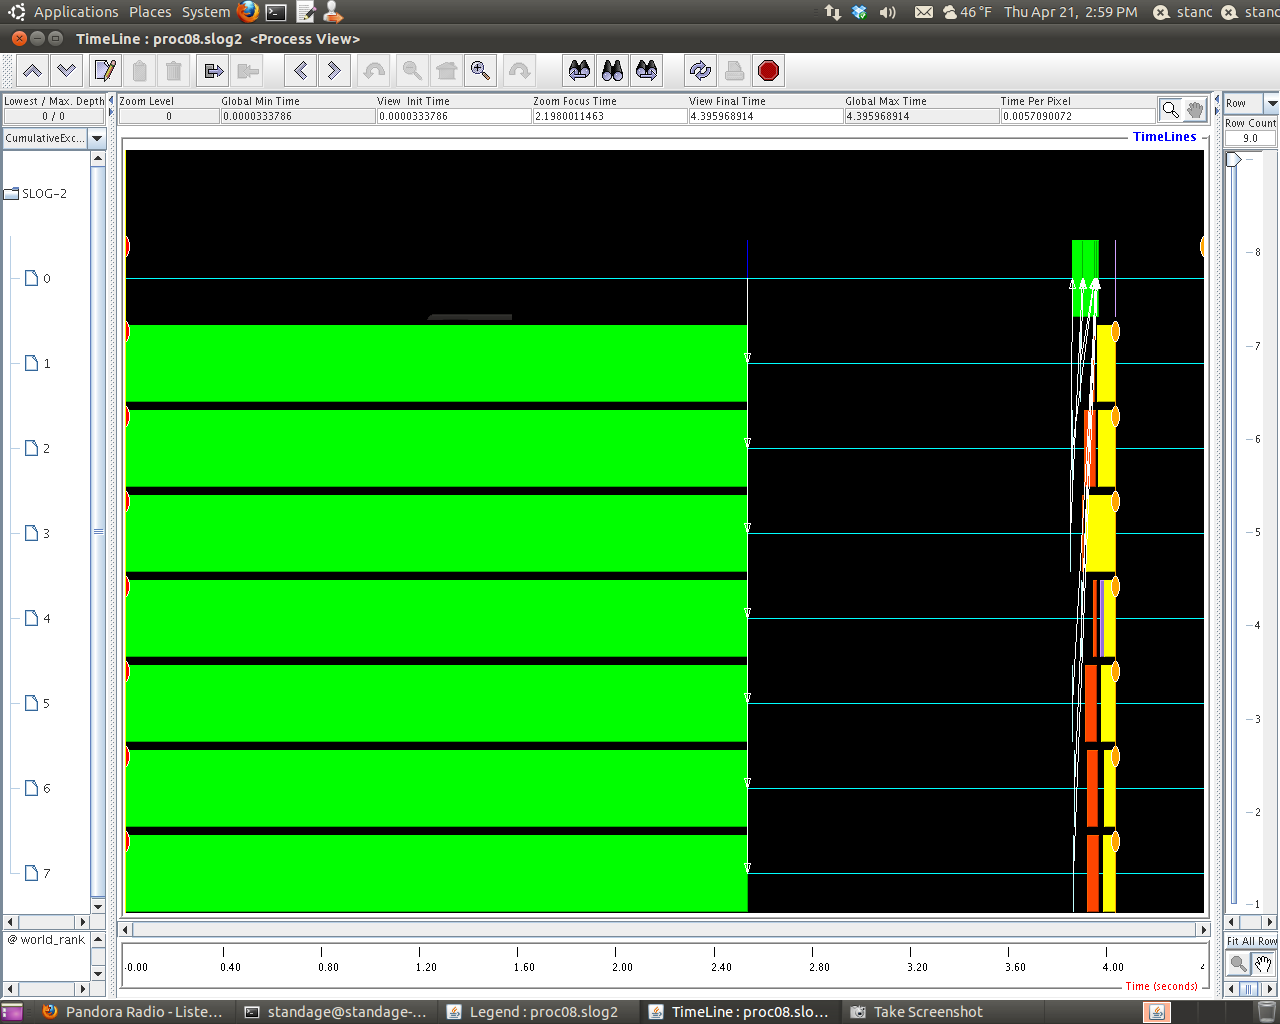
\includegraphics[height=200px]{procs-08.png}
    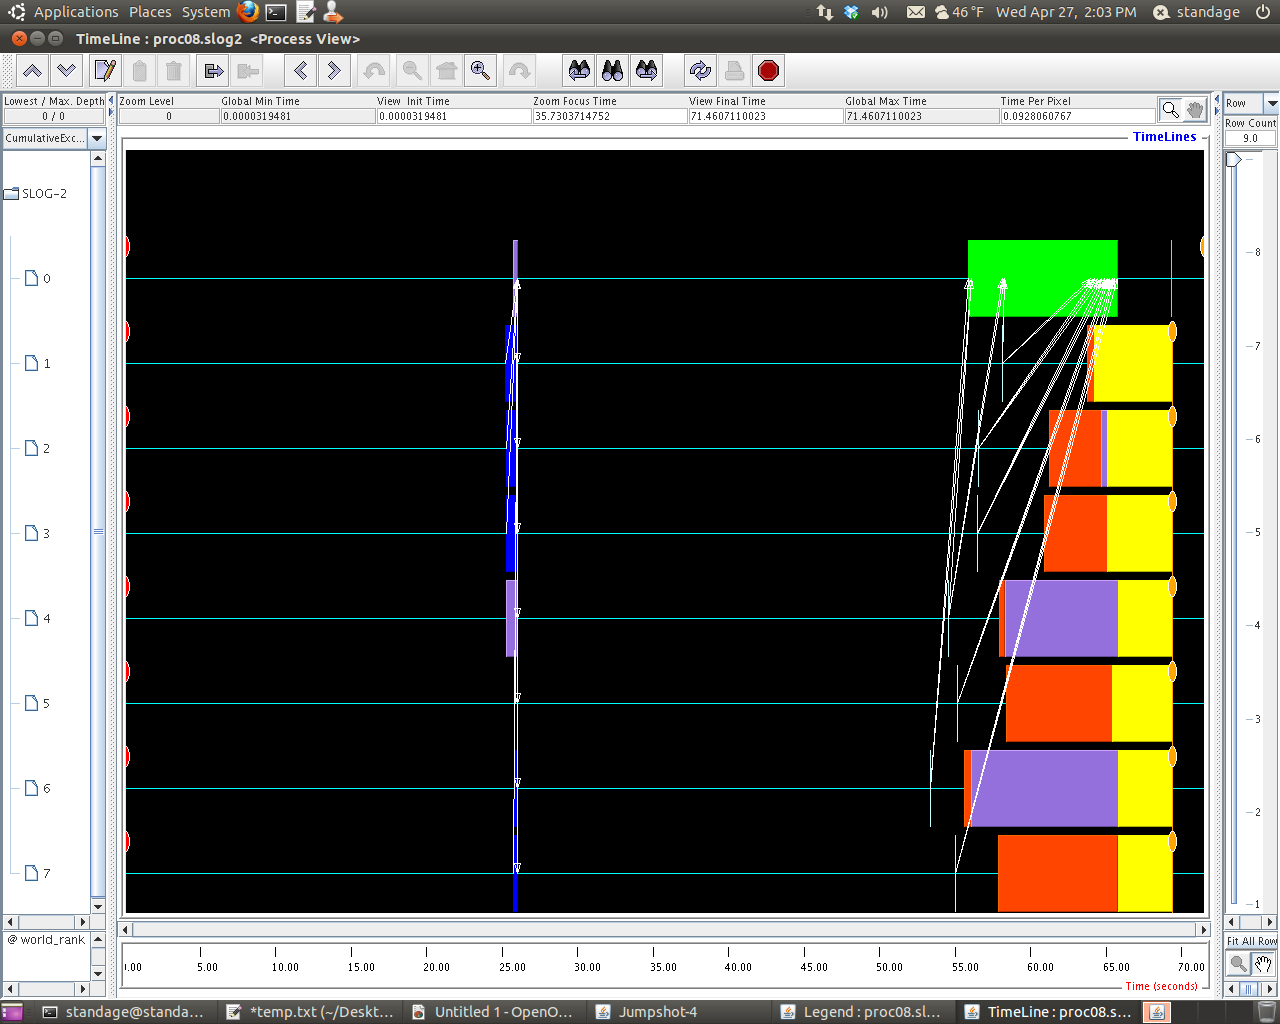
\includegraphics[height=200px]{proc08-hg.png}
  \end{center}
  \caption{MPI trace visualizations for ParsEvalMPI before (left) and after (right) an improvement in the delegation phase's implementation. Initially, the delegation phase of the ParsEvalMPI program was executed serially on the root processor. As a result, all other processors were idle for approximately half of the program's runtime (the green bars on the left represent idle time spent in the \texttt{MPI\_Recv} routine). After the delegation phase was re-implemented, the runtime and idle time were significantly reduced, improving the performance and load balancing. Here, 8 processors are shown, but results are similar for 2, 4, 8, 16, and 32 processors.}
\end{figure*}

\subsection*{Local analysis}
The purpose of the local analysis phase is to analyze each gene locus, comparing the corresponding predictions from the two sets of annotations. In the previous delegation phase, the program determines the optimal distribution of data and work. In the local analysis phase, each processor works independently to analyze its delegated region.

The first step in the comparison is the generation of two \textit{model vectors}. Each processor must first generate two model vectors (corresponding to the two sets of annotations) for its locally delegated region of the DNA sequence before performing the comparative analysis. Once the model vector is generated, each processor sends its two model vectors to the root processor using non-blocking sends. The model vectors do not need to be modified once they are created, so there are no potential issues with overlapping the send routines and the comparison routines. This overlap provides a slight performance improvement.

While the non-blocking send it pending, each processor continues with the comparative analysis, printing detailed comparison statistics for each gene locus to an output file.

\subsection*{Global analysis}
The purpose of the global analysis phase is to provide a brief summary analysis of the entire DNA sequence. The analysis itself is not easily parallelized, but it does rely on the model vectors generated in parallel during the local analysis phase. Once the initial delegation phase is complete, the root processor (along with all other processors) is delegated a region of the DNA to analyze. The root processor begins, like all other processors, by generating a model vector for its delegated region of the DNA. However, instead of performing a non-blocking send and moving on to analysis (as do the other processors), the root processor receives model vectors from each processor. Then when the local analysis phase is complete, the root processor does a brief analysis of the entire DNA sequence and prints some summary statistics.

\subsection*{Serial optimizations}
When possible, ParsEvalMPI uses native data types and static arrays for storing data, and stride-1 array access for retrieving data. However, the format of data files used to store gene structure annotations is quite complex and is impossible to parse without the use of dynamic data structures. Unfortunately, these data structures introduce some overhead, especially when iterating over a dynamic list whose elements are not contiguous in memory. Additionally, when these data needed to be shared between processors, the program had to copy the data from the dynamic structures to arrays that can be sent using MPI routines, introducing even more overhead. To reduce the overhead corresponding to dynamic data structures, they were only used when absolutely necessary.

\end{methods}

\section*{Results} 
\subsection*{Improvement over serial program}
ParsEvalMPI represents a significant improvement over ParsEval in terms of memory usage and (especially) overall runtime. To demonstrate this improvement, I ran ParsEvalMPI on two pairs of gene structure annotations. The reduced memory usage was consistent but difficult to quantify. An evaluation of the runtimes, however, is provided hereafter.

In the first analysis, ParsEvalMPI compared gene structure annotations for chromosome 1 of \textit{Arabidopsis thaliana} between TAIR versions 9 and 10 (see \url{http://arabidopsis.org/}). This analysis required only 4-6 seconds to complete with ParsEvalMPI, a huge improvement over the previous version of ParsEval, which required between 20-40 minutes of runtime.

In the second analysis, ParsEvalMPI compared gene structure annotations for the entire human genome between versions 61 and 62 (respectively) of the Ensembl GRCh37 human genome gene build (see \url{http://gremlin4.gdcb.iastate.edu/~standage/blog/?p=329}). This analysis required 1-2 minutes to complete, which represents a huge improvement over the previous version of ParsEval which could not even handle a data set of that size.

\subsection*{Data distribution and load balancing}
The \textit{delegation} phase of the program ensures that the data and compute time are distributed optimally between the \textit{p} processors. Although the initial implementation of the delegation phase led to serious issues with load balancing, the updated implementation yielded very good distribution of data and work among the processors throughout the entire program's runtime (see \textbf{Fig. 2}).

\subsection*{Scalability}
While the overall performance of ParsEvalMPI is a huge improvement over the previous serial version, the scalability of ParsEvalMPI is nevertheless poor. Tests suggest that the maximum speedup factor for ParsEvalMPI approaches a value of 2.
\begin{figure*}
  \begin{center}
    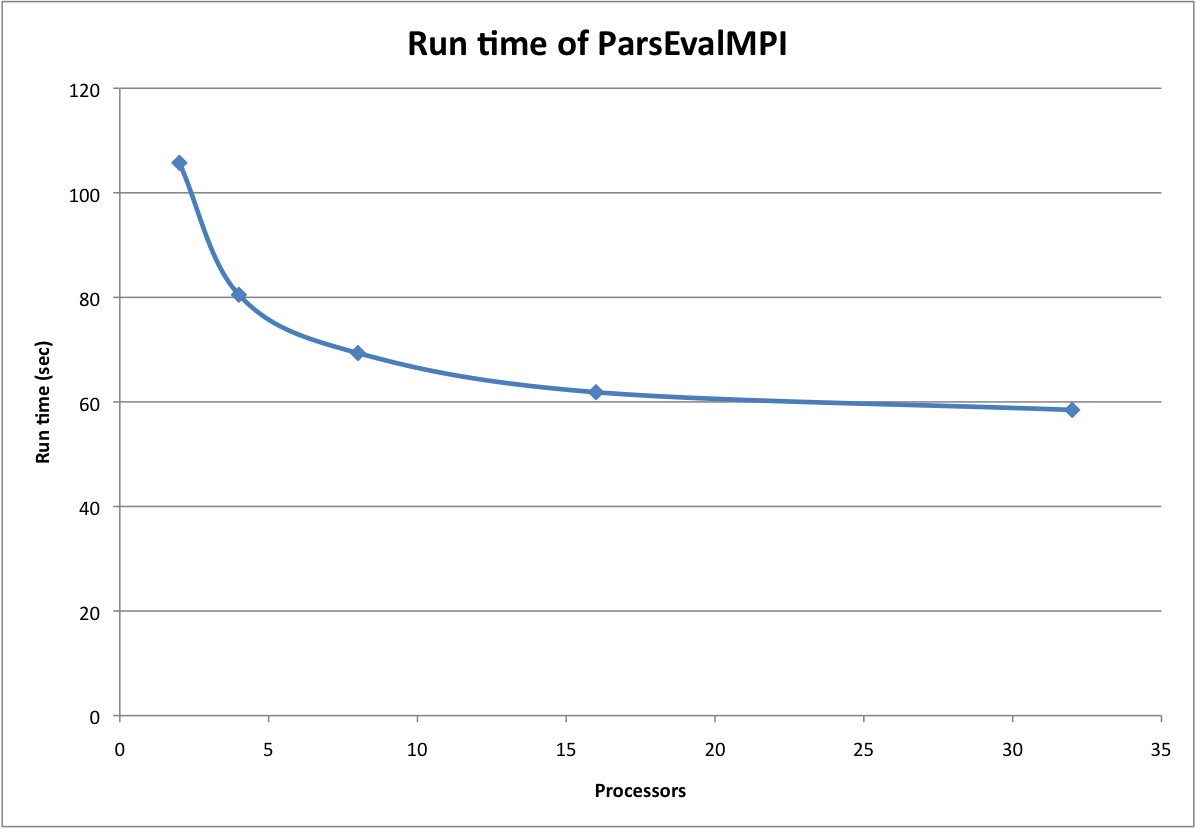
\includegraphics[height=150px]{runtime.png}
    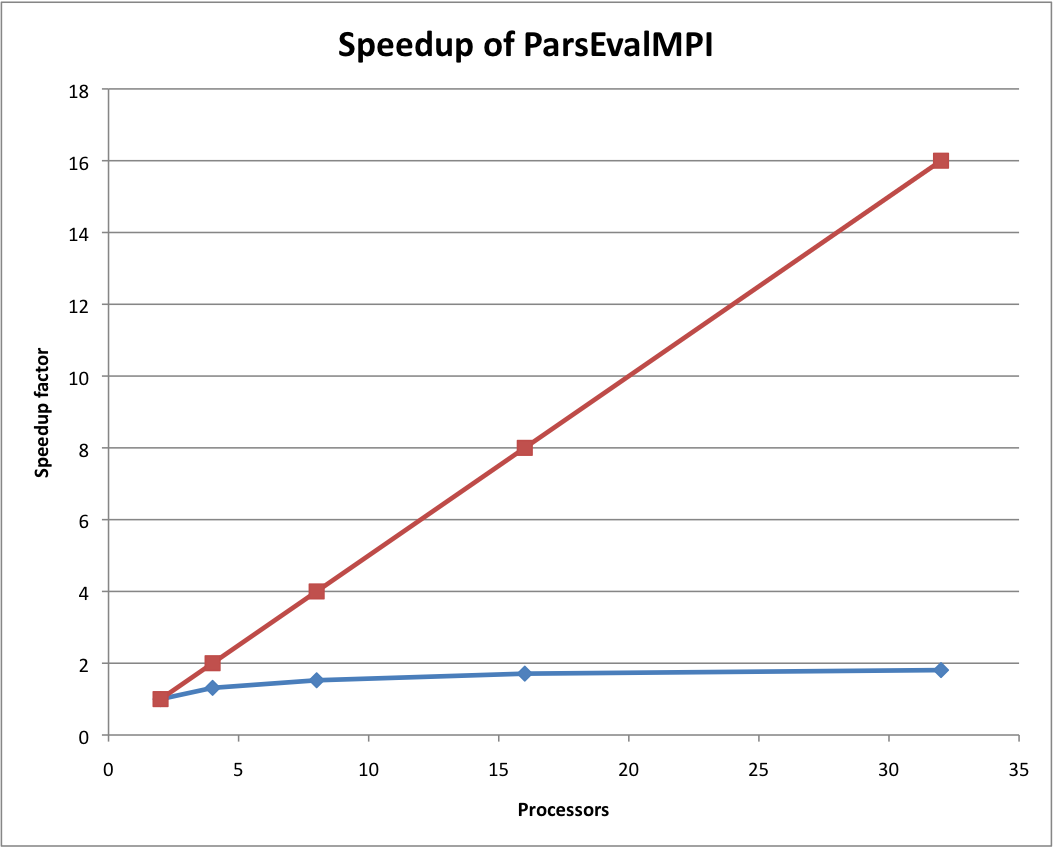
\includegraphics[height=150px]{speedup.png}
  \end{center}
  \caption{Unfortunately, ParsEvalMPI has very poor scalability, approaching a speedup factor of only 2. The graph on the left shows the runtime of the program with the size of the data set fixed. The graph on the right shows the desired speedup in red and the actual speedup achieved by ParsEvalMPI in blue.}
\end{figure*}

\section*{Discussion}
Comparing gene structure annotations is an important aspect of my research, and ParsEvalMPI provides the most efficient solution for performing this type of analysis. Implementing the program in C and taking advantage of the MPI libraries provides huge performance improvements over the serial version I previously developed. By implementing a delegation phase, I ensured an even distribution of data and work amongst the processors, reducing processor idle time. Despite the excellent data distribution and load balancing, ParsEvalMPI nevertheless has very poor scaling properties, approaching a speedup factor of only 2. I have still been unable to determine the reason for this, but I have considered trying to implement the program using OpenMP and the shared memory paradigm, which may yield better results. Regardless, I am very happy to be able to compare gene structure annotations so quickly and efficiently.

%\begin{thebibliography}{}
%\begin{raggedright}
%\bibitem[Dong \textit{et~al}, 2004]{Dong04} Dong Q., Schlueter S.D., and Brendel, V. (2004) PlantGDB, plant genome database and analysis tools. \textit{Nucleic Acids Research}, \textbf{32}, D354-D359.
%
%\bibitem[Farlow \textit{et~al}, 2010]{Farlow10} Farlow A., Meduri E., and Schlotterer C. (2010) DNA double-strand break repair and the evolution of intron density. \textit{Trends in Genetics}, In Press, Corrected Proof, Available online at \url{http://www.sciencedirect.com/science/article/B6TCY-51J095Y-1/2/e315164099aa37405e3ca29d32f06fbf}.
%
%\bibitem[Fedorov \textit{et~al}, 2001]{Federov01} Fedorov A., Cao X., Saxonov S., de Souza S.J., Roy S.W., and Gilbert W. (2001) Intron distribution difference for 276 ancient and 131 modern genes suggests the existence of ancient introns. \textit{Proceedings of the National Academy of Sciences of the United States of America}, \textbf{98}, pp. 13177-13182.
%
%\bibitem[Fedorov \textit{et~al}, 2002]{Federov02} Fedorov A., Merican A.F., and Gilbert W. (2002) Large-scale comparison of intron positions among animal, plant, and fungal genes. \textit{Proceedings of the National Academy of Sciences of the United States of America}, \textbf{99 (25)}, pp. 16128-16133.
%
%\bibitem[Gilbert, 1978]{Gilbert78} Gilbert W. (1978). Why genes in pieces? \textit{Nature}, \textbf{271(5645)}, p. 501.
%
%\bibitem[Rogozin \textit{et~al}, 2003]{Rogozin03} Rogozin I.B., Wolf Y.I., Sorokin A.V., Mirkin B.G., Koonin E.V. (2003) Remarkable interkingdom conservation of intron positions and massive, lineage-specific intron loss and gain in eukaryotic evolution. \textit{Current Biology}, \textbf{13 (17)}, pp. 1512-1517.
%
%\bibitem[Roy and Gilbert, 2005]{Roy05} Roy S.W., Gilbert W. (2005) Complex early genes. \textit{Proceedings of the National Academy of Sciences of the United States of America}, \textbf{102 (6)}, pp. 1986-1991.
%
%\bibitem[Wang \textit{et~al}, 2003]{Wang03} Wang C., Li Z., Typas M.A., Butt T.M. (2003) Nuclear large subunit rDNA group I intron distribution in a population of Beauveria bassiana strains: phylogenetic implications. \textit{Mycological Research}, \textbf{107(10)}, pp. 1189-1200.
%\end{raggedright}
%\end{thebibliography}

\end{document}
